\chapter{関連研究}
本研究では,深層能動学習によってアノテーションコストを抑えつつ大規模病理画像解析を行うためのシステムを構築する.
本章では,それらに関連する研究の枠組みについて述べる.
2.1節では画像認識で目覚ましい成果を挙げている深層学習において,汎化性能を向上させるためのいくつかの工夫について述べる.
2.2節では病理画像解析の性質と先行研究について説明する.
2.3節では能動学習に関する基本的な概念について説明する.
2.4節では本研究に関連する先行研究を概観し,本研究の位置付けを述べる.

\section{画像認識における深層学習}
\subsection{概観}
深層学習とは,多層のニューラルネットワークを用いて高い識別性能を達成するモデルを構築する機械学習技術の1つである.
Convolutional Neural Network (CNN)とは,画像認識分野において近年目覚ましい成果を挙げている多層ニューラルネットワークである.
2012年に大規模一般画像認識のコンペティションであるILSVRC\cite{ILSVRC15}でCNNを用いたチームが優勝して以来,画像に関する様々なタスクにおいて利用されている.
従来の画像認識では,画像を認識するために有効だと考えられる特徴量を人手で設計し,
その特徴量を用いて識別器を学習するというフレームワークであったのに対し,CNNは学習の過程で訓練データから識別に有効な特徴量を抽出する表現学習と,その特徴量の識別境界を決定する識別器の学習が同時に行われる点で特徴的である.

しかし一般に,CNNは非常に過学習に陥りやすく,大量のラベルつきデータセットを構築する必要があることが知られている.
また,十分なデータ量がある場合でも,高い汎化性能を持つCNNを学習させるにはいくつかの工夫を追加することが多い.
本節の残りでは,それらの工夫の中でも本研究に関連するものについて説明する.

\subsection{\textbf{Dropout}}
一般に機械学習では,訓練データに対する過学習を防ぎ汎化性能を向上させるために,モデルの正則化が行われる.
ニューラルネットワークの正則化手法の1つにDropout\cite{hinton2012improving, srivastava2014dropout}がある.
Dropoutとは,学習の過程において,ニューラルネットワークの中間層のニューロンを一定確率でランダムに"drop"する,すなわち出力を0にする正則化手法である(図. \ref{fig:dropout_network}).
これは,任意の$n$次元中間層の出力$y_i$に対し,以下のようなマスク$M$との要素積$\otimes$を取ることで行われる.
\begin{eqnarray*}
    y'_i &= y_i \otimes M 
\end{eqnarray*}
\begin{eqnarray*}
    M &= [m_0, m_1, \dots, m_n],\;\; m_i \sim Bernoulli(\pi) 
\end{eqnarray*}
$y'_i$は次の層への入力として使用される.$m_i$はそれぞれ,パラメータ$\pi$のベルヌーイ分布から順伝播毎にサンプリングされる値である.

\begin{figure}[tbp]
    \begin{minipage}{0.5\hsize}
     \begin{center}
      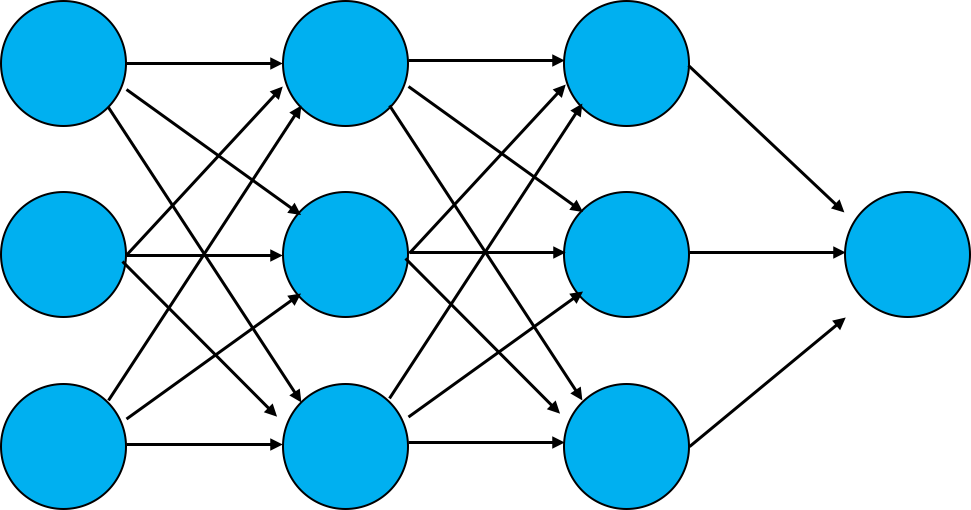
\includegraphics[width=60mm]{figures/standard_network.png}
     \end{center}
     \label{fig:one}
    \end{minipage}
    \begin{minipage}{0.5\hsize}
     \begin{center}
      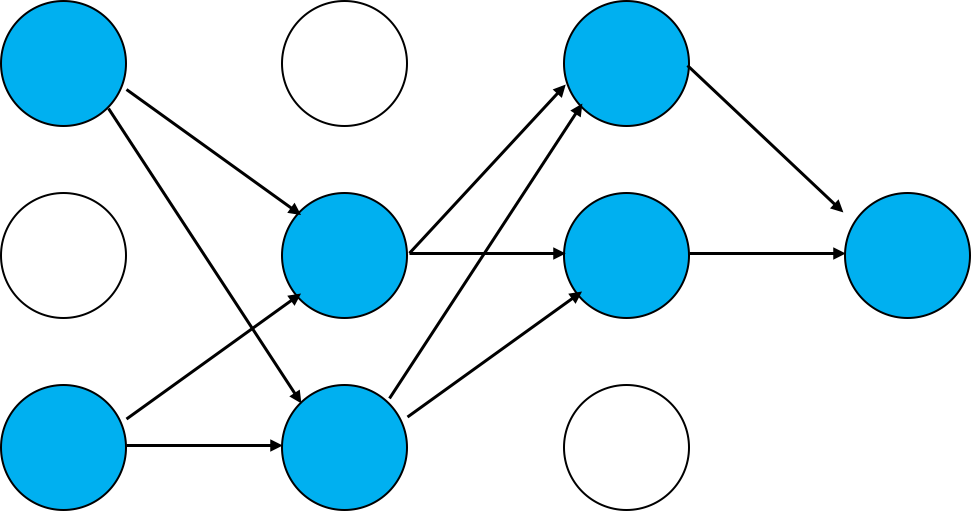
\includegraphics[width=60mm]{figures/dropout_network.png}
     \end{center}
     \label{fig:two}
    \end{minipage}
    \caption{\label{fig:dropout_network}Dropoutの模式図.(左)通常のネットワーク (右)いくつかのニューロンがDropされたネットワーク}
    
\end{figure}

これにより,あるニューロンが特定のニューロンにのみ過剰に依存してしまう共適合(Co-adaptation)を防ぐことができる.
また,指数的組み合わせの数の部分ネットワークを同時に学習していると見なすこともでき,
複数の部分ネットワークのアンサンブルを行っているのと同じ効果があるとも見なすことが出来る.

\subsection{\textbf{Data Augmentation}}

Data Augmentationとは,画像識別問題においてニューラルネットワークの汎化性能を向上させるために利用される手法である.
訓練時に使用する画像に対し,ラベル情報を保持する程度の変形(主に幾何学的変形)を加えたものを入力して学習を行うことで,
画像の様々な変形に対し不変な特徴量を抽出して予測をすることを期待するものである.
モデルに回転不変性を与えるために元画像に回転を加える,位置不変性を与えるために元画像に平行移動を加える等の変形がしばしば用いられる.
例を図\ref{fig:data_augmentation}に示す.

\begin{figure}[tbp]
     \begin{center}
      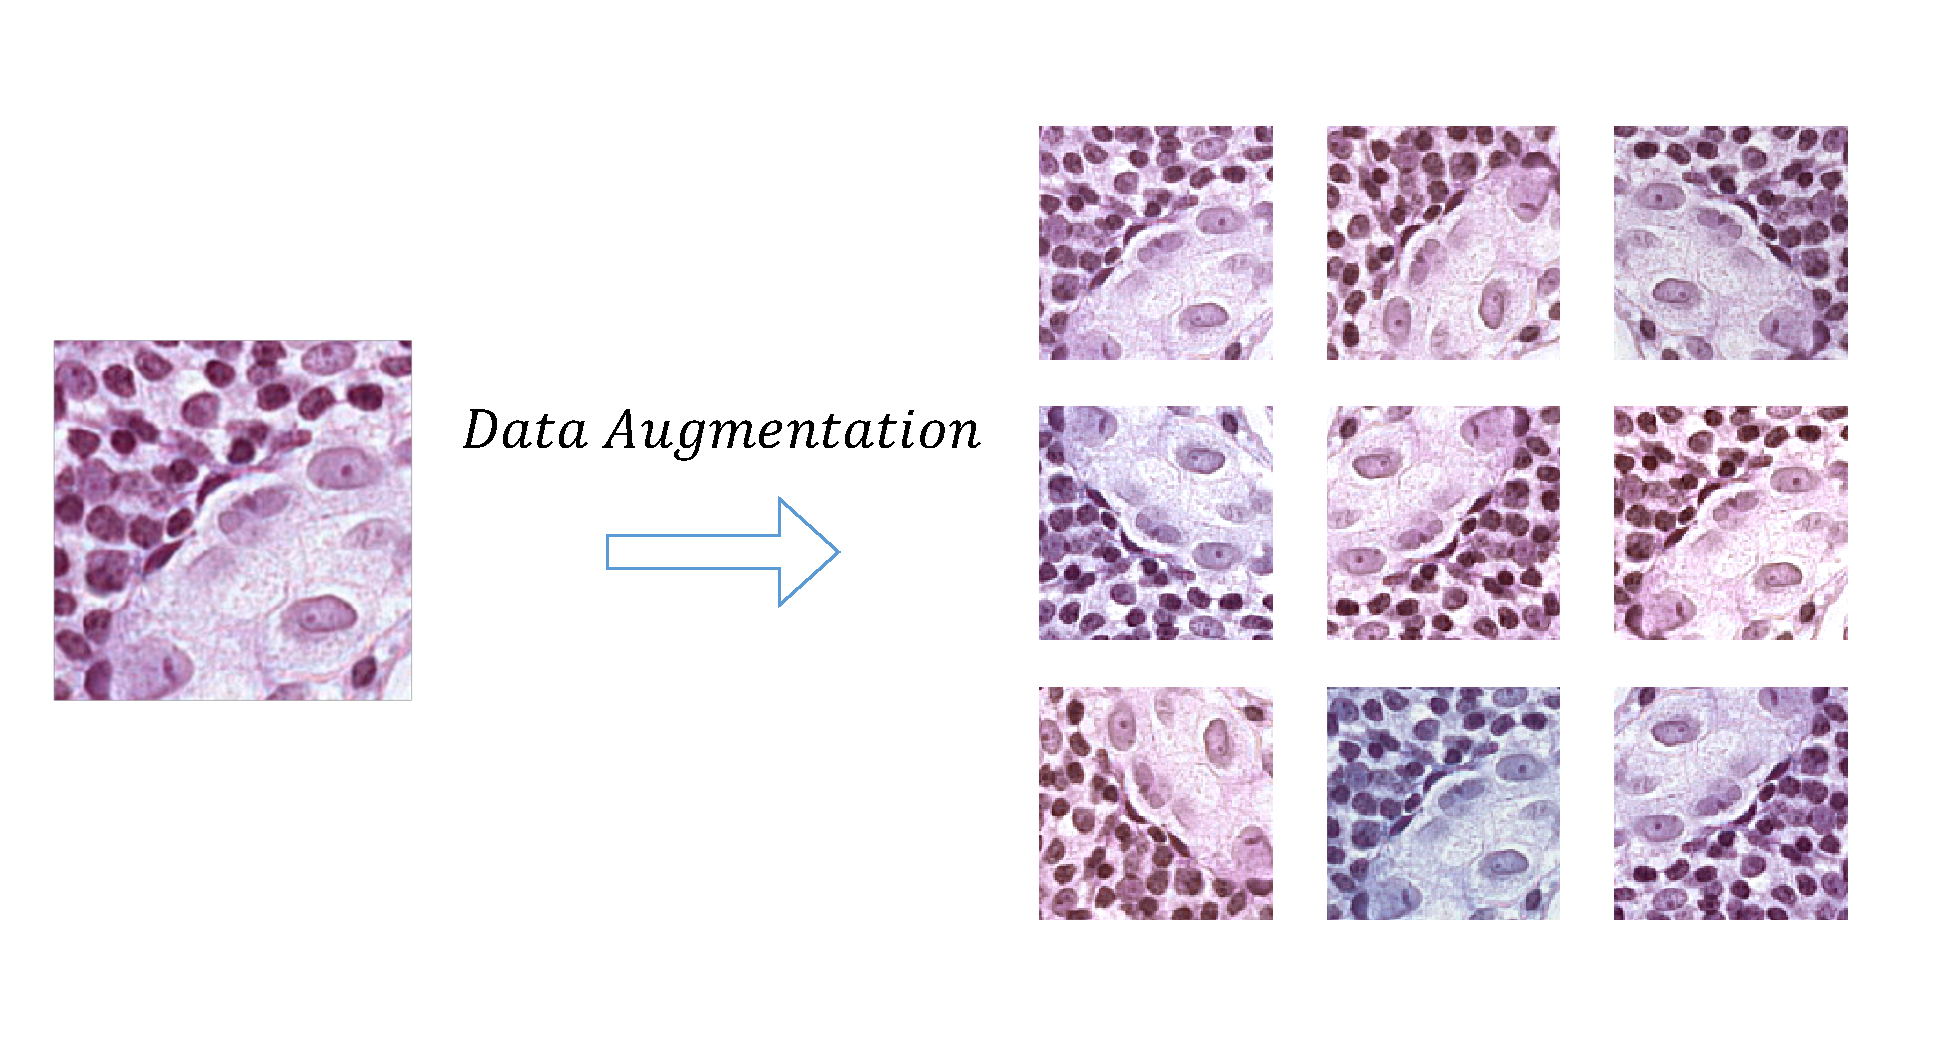
\includegraphics[width=12cm]{figures/data_augmentation.pdf}
     \end{center}
    \caption{\label{fig:data_augmentation}1枚の病理画像パッチに対してData Augmentationを行った例.ここでは,Random Crop,Random Rotation,Random Flip,Random Color Augmentationを使用した.}
\end{figure}

\subsection{学習済みモデルからの転移学習}
\label{sec:transfer}
転移学習とは,ある問題を効率的に解くために,別の関連した問題のデータや学習結果を再利用する枠組みである.
深層学習における転移学習とは,しばしばfine-tuningによるものを指すことが多い.
fine-tuningとは,ニューラルネットワークを学習するために別のタスクもしくは別のデータセットで学習済みのモデルを初期値として利用して再学習を行うことである.
特に,大規模一般画像認識データセットであるImageNet\cite{imagenet_cvpr09}の学習済みモデルをfine-tuningさせることで,
幅広い画像認識タスクにおいて従来の手法と比較して高い性能を達成することが知られている\cite{girshick2014rich, agrawal2014analyzing}.
また,fine-tuningの場合,比較的少数の訓練データからでも優れた性能が得られることが示されている.

\section{病理画像解析}
\label{sec:path_images}
本節では,病理画像解析の性質と関連研究を述べる.

\subsection{概観}
第1章で述べたように,病理画像とはWSIと呼ばれる巨大なデジタル画像のことを指す.
病理画像解析におけるアプリケーションは,大きく分けて以下の3つに分類される\cite{komuraishikawa}.
\begin{itemize}
    \item 自動診断による医師の補助
    \item 類似画像検索による医師の補助
    \item 画像と画像以外の情報(分子構造,遺伝子情報など)との関連性の解析
\end{itemize}
中でも,近年の画像認識技術の向上により自動診断に関する研究が急速に増加している\cite{doyle2008automated,dundar2011computerized}.
本研究でも,自動診断に位置づけられる癌(異常)の自動検知タスクに焦点を当てる.

\begin{figure}[tbp]
    \label{fig:path_images}
     \begin{center}
      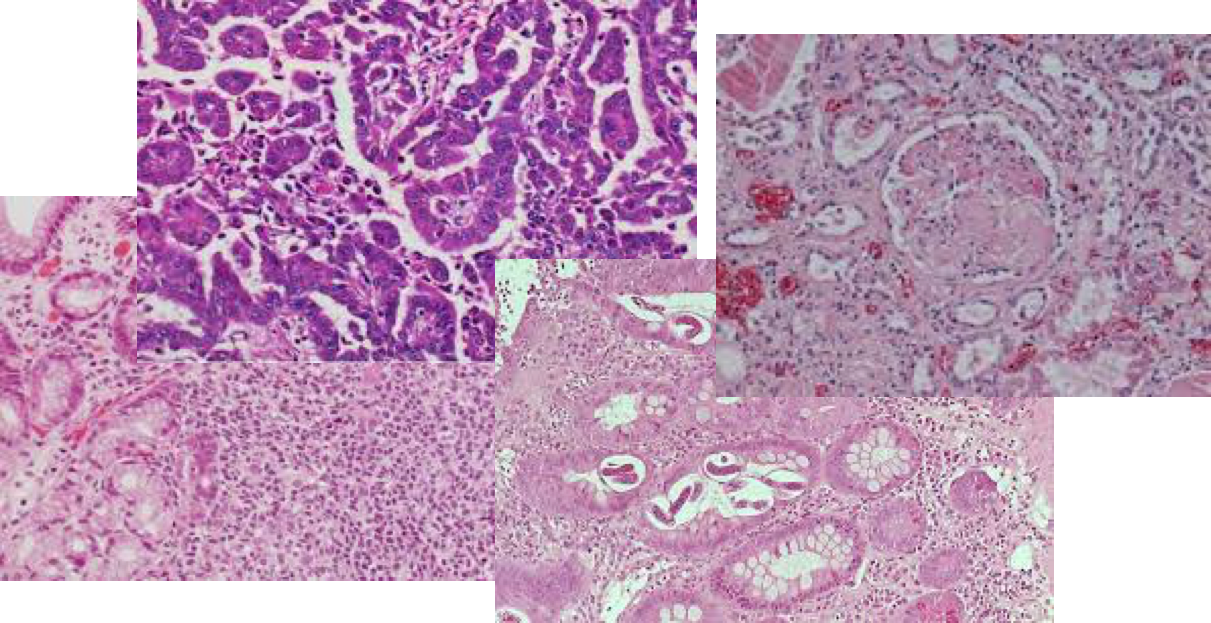
\includegraphics[width=13cm]{figures/path_images.png}
     \end{center}
    \caption{病理画像の例.}
\end{figure}
    
\subsection{WSI全体の予測の出力方法}
一般に,画像認識タスクにおいて用いられる画像は高々1000×1000以下である.
数万ピクセル×数万ピクセルに及ぶWSIの全ピクセルを1つのモデルに入力して一度に学習を行うのはデータ数,パラメータ数,どちらの面においても現実的ではない.
また,癌などの異常部位というのはWSIのわずか領域にのみ現れることも多く,解像度を落として使用しても期待する性能が得られない.
そのため,多くの病理画像解析では,WSIを大量の画像パッチ(1000×1000以下)に分割し,それぞれを個別に識別した結果を統合することで癌の有無を判定することが多い.
個々の画像パッチを識別するモデルは,一般的な画像認識タスクで用いられるものを使用する.

\subsection{使用される画像特徴量および識別器}
画像認識において特徴量抽出は重要な役割を持つ.
一般に医療画像解析では,一般画像認識に使用されるSIFTなどのhand-craftedの画像特徴量が同様に利用されていた\cite{caicedo2009histopathology}.
また,病理画像は特定のオブジェクトが存在するか否かというよりも,画像全体の模様,もしくはテクスチャとしての性質を持つことから,HLAC, LBPなどのテクスチャ解析における手法を採用する研究も盛んに行われていた\cite{sertel2008texture, sertel2009histopathological, nosato2011extended}.
ただ,近年では一般画像認識における深層学習の成果を受けて,CNNを採用する研究が大半を占める\cite{hou2016patch, xu2016deep, litjens2016deep, chen2016dcan, liu2017detecting}.
またCNNを利用する研究の中では,病変の検出率\cite{liu2017detecting}や癌の識別率\cite{xu2016deep}が病理医に匹敵,あるいは超えるほどの精度を達成したという報告もある.

一般画像認識と比較して多くの医療画像解析ではラベル付きデータが少ないことから,
ImageNetなどのデータセットをpretrained-modelの中間特徴量を抽出し識別器はSVMなどを利用する場合や,
\ref{sec:transfer}で述べたような転移学習を利用する場合がある.
直観に反し,それらの中間特徴量は一般画像を認識するために学習されたものであっても,
医療画像解析でも十分な性能を達成することができることが知られている\cite{li2014medical, tajbakhsh2016convolutional}

\subsection{病理画像解析特有の性質}
一般に医療画像解析に共通している特徴として,モデルが画像に対して獲得すべき不変性が多いということがある.
特に病理画像解析では,各画像パッチは人手で切り取られたものであるので,モデルの予測は回転,位置に対しては不変であることが強く求められる.
また,病理画像はそもそも染色液によって細胞を染色することで核などの病理学的特徴を見つけ出すための画像であるが,
その染まり方は細胞毎,研究機関毎に大きく異なる(図\ref{fig:comparison_color}).
このことから,色相,輝度に対する不変性が強く必要とされる.

\begin{figure}[tbp]
     \begin{center}
      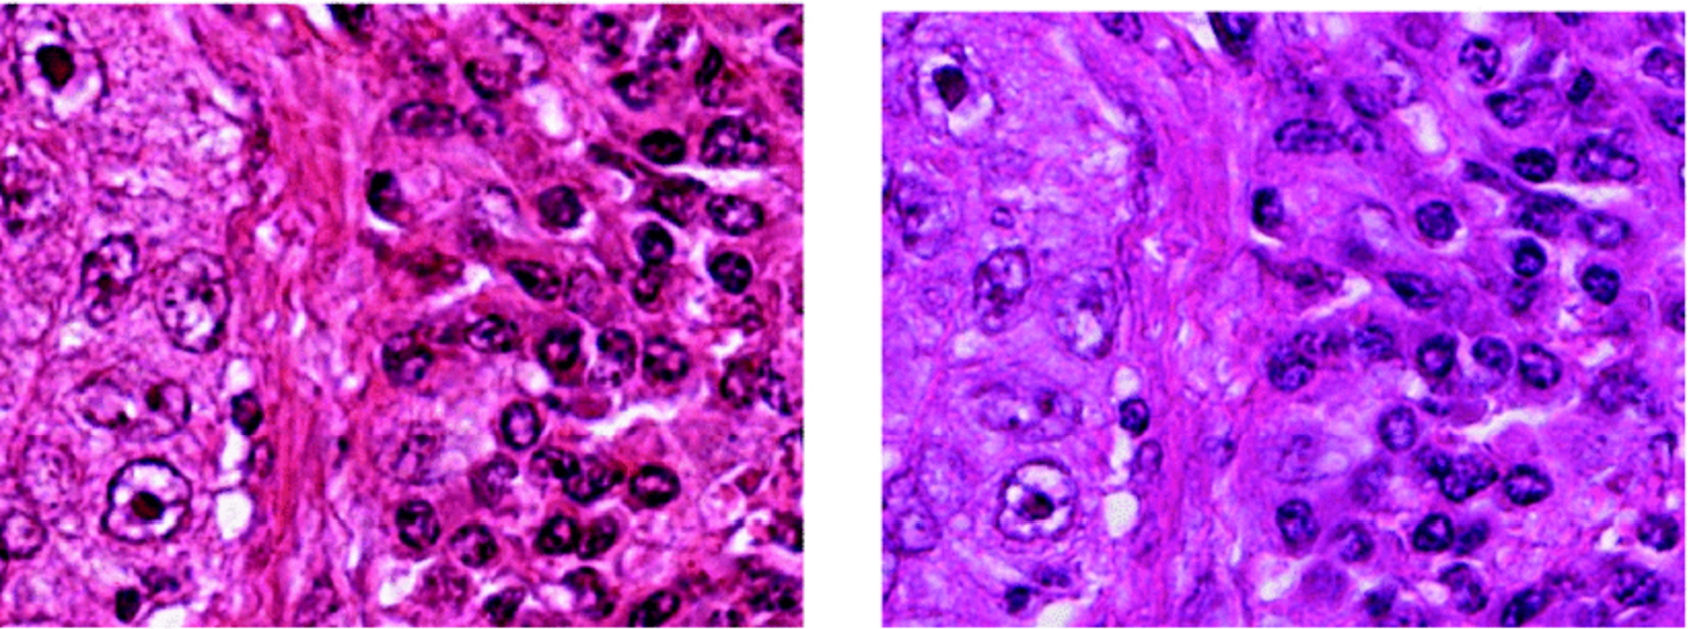
\includegraphics[width=13cm]{figures/comparison_color.pdf}
     \end{center}
    \caption{\label{fig:comparison_color}同じ細胞組織を異なる細胞スキャナーによって撮像したもの.色,解像度,輝度に大きな変化があることがわかる.}
        % ICPR 2014 MITOS-atypia challenge—http://mitos-atypia-14.grand-challenge.org
\end{figure}

\section{能動学習}
\label{seq:al}
この節では,能動学習についての基本的な概念および先行研究について述べる.

\subsection{基本的な概念}
能動学習(Active Learning)\cite{settles2010active}とは,機械学習における1つの枠組みである.
一般に,教師つき学習において識別精度の高いモデルを学習させるためには膨大なラベル付きデータが必要となる.
そこで,能動学習では,与えられる大量のラベルなしデータから,モデルの更新に最も寄与する可能性のあるサンプルを選択し,
それにアノテーションを付与することで,低いアノテーションコストのもとでいかに高精度な予測モデルを作成するかを目的としている.
データ自体は豊富にあるが,アノテーション付与のコストが高価であるような問題に用いられる.

能動学習の基本的な流れを以下に示す
\begin{itemize}
    \item[1.] モデル更新に寄与する可能性のあるサンプルを選択 (クエリ選択)
    \item[2.] 専門家によってアノテーションを付与 (クエリ問い合わせ)
    \item[3.] 付与されたアノテーションを利用し教師あり学習を実行 (再学習)
\end{itemize}
通常,学習が飽和するまでこれらのサイクルを繰り返す.以下それぞれのステップについて詳細を述べる.
クエリ選択の詳細については次項で詳細を述べる. 

クエリ問い合わせについて,学習主体がクエリを問い合わせる問題設定は以下の3種類に大別される
\begin{description}
    \item[Stream-Based Selective Sampling]\mbox{}\\
        ストリーミングデータ (サンプルが次々に入力されていくような場合) に対するアプローチ.
        入力されるストリーミングデータに対してラベルを付けるかを逐一判断し,
        モデル更新に寄与すると判断された場合(大抵は閾値を設ける),クエリとして問い合わせる方式である.
    \item[Pool-Based Sampling]\mbox{}\\
        巨大なラベル無しデータ集合(サンプルプール)が予め与えられている問題に対するアプローチである.
        ストリーミングデータの場合とは違い,閾値を設けることなくプールの中から最もモデル更新に寄与するサンプルを選択することができる.
        また,サンプルデータの分布,およびデータ構造を考慮したクエリ選択が可能となる.
    \item[Membership Query Synthesis]\mbox{}\\ 
        ストリーミングデータ,プールサンプルどちらの状況でも利用され,
        実際のデータを直接クエリとして利用するのではなく1つまたは複数のサンプルから新しい人工データを生成し
        人間に提示する事でラベル付けを行う方法である.
\end{description}
中でも,Pool-based Samplingの問題設定での研究が最も行われている.
病理画像解析ではラベルが付与されていないWSIおよびそれに含まれる画像パッチは大量にある場合がほとんどであるため,
本研究でも,ラベルなしサンプルプールが予め与えられているPool-based Samplingの問題設定を採用する.

再学習について,能動学習の研究では二通りの方法がある.
1つは,クエリ問い合わせによってラベル付きデータが追加する度に,識別器のパラメータを初期値に戻してから再学習を行う方法である.
ラベル付きデータが増える度にスクラッチ学習を行うため,クエリ問い合わせ間隔が大きくなってしまう欠点がある.
もう1つは,識別機のパラメータを初期値に戻すことなく,継続的に学習を行う方法である.
ナイーブに学習を行うと,学習初期にラベルを付与されたデータの影響が大きくなってしまうため,新しいラベル付きデータに重みをつけて学習を行うなどの調整が必要となる.
多くの研究では,再学習に時間のかからない線形識別器を用いているため,1つ目の再学習手法が採用される.
識別器にCNNを用いた場合再学習に時間がかかってしまうが,ハイパーパラメータ数の削減や学習の安定性という観点から,本研究でも再学習毎に識別器のパラメータを初期値に戻す方法を採用する.

\subsection{クエリ選択の基準}
\label{query_strategy}
本項では,モデル更新に寄与する可能性が高いと判断する基準(クエリ選考基準)として提案されているいくつかのものについて述べる.
$\mathcal{L}$をラベル付きデータセット,$\mathcal{U}$をラベルなしデータセットとする.
クエリはそれぞれの選考基準で使用されるスコアリング関数を最大にするサンプルを選択するものとする.
\begin{eqnarray}
    x^{*} = \argmax_{x \in \mathcal{U}} \: score(x)
\end{eqnarray}
また,識別器のパラメータを$\theta$とし,サンプル$x$が与えられた時のクラスラベル$y$の予測確率を$P_{\theta}(y|x)$とする.

\subsubsection{Uncertainty Sampling \cite{lewis1994sequential}} 
最もシンプルな戦略で,モデルにとって予測が最も曖昧であるようなサンプルをクエリとして選択する.
データ$x$が与えられた時,ラベルの確率分布$p(y|x)$を出力する識別器であればいいという緩い条件のため幅広く利用されている.
曖昧性の定量評価として,
事後確率最大ラベルの確率が小さいサンプルを選択するLeast Confident(式\ref{eq:least_confident}),
事後確率最大ラベルの確率と,その次に大きなラベルの確率との差が小さいサンプルを選択するMargin Sampling(式\ref{eq:margin}),
事後確率分布のエントロピーが大きいサンプルを選択するEntropy Sampling(式\ref{eq:entropy})
などが提案されている.
\begin{eqnarray}
    score(x) &=& 1 - P_{\theta}(\hat{y}|x)  \;\;  \label{eq:least_confident} \\ \nonumber \\ 
    score(x) &=& - (P_{\theta}(\hat{y}_1|x) - P_{\theta}(\hat{y}_2|x) )  \;\;  \label{eq:margin}\\ \nonumber \\
    score(x) &=& - \sum_i {P_{\theta}(y_i|x)} \log P_{\theta}(y|x)  \;\;  \label{eq:entropy}
\end{eqnarray}
多値分類の際はこれらはそれぞれ性質の異なるものになるが,二値分類の場合は全て等価な戦略となる.

\subsubsection{Query-By-Committee \cite{seung1992query}}
モデルの仮説空間内で,現在のラベル付きデータに対してConsistentな領域をバージョン空間と呼び,バージョン空間が大きいほどパラメータの推定の分散が大きいことを示す.
そこで,バージョン空間を縮小させるサンプルがモデルの更新に寄与するはずだとする仮説に基づく戦略がある.
実際にバージョン空間をすべて保持することは現実的には不可能であるため,近似的にこれを扱うための手法がいくつか提案されている.
その中で代表的な手法がQuery-By-Committee(QBC)アルゴリズム\cite{seung1992query}である.
バージョン空間を近似的に表現するために,現在のラベル付きデータ集合を使用して学習した
複数のモデル(Committee $C=\{ \theta^{(1)}, \dots, \theta^{(C)}\}$)を保持し,
Committee内のメンバの予測の不一致度が最も高いサンプルを選択するという戦略である.
不一致度の定量評価として,Vote Entropy \cite{dagan1995committee},Average Kullback Leibler Divergence \cite{mccallum1998employing}がある.
Vote Entropyは,Committee内のメンバがどのラベルだと予測(投票)したかのばらつきを定量化したもので,次式で表される
\begin{eqnarray}
    score(x) =  - \sum_{j=1}^{m} \frac{V(y_j)}{|C|} \log \, \frac{V(y_j)}{|C|}
\end{eqnarray}
$V(y_j)$はクラス$j$の得票数,$|C|$はCommitteeのサイズを表す.

Average Kullback Leibler Divergenceは,それぞれ予測分布の確率分布の差異が平均的に大きいものを選ぶ手法である.
\begin{eqnarray}
    score(x) =  -  \frac{1}{|C|} \sum_{c=1}^{|C|} KL \, (P_{\theta^{(c)}} || P_{C})
\end{eqnarray}
$P_{\theta^{(c)}}$は$c$番目のCommitteeの確率分布, $P_C$はCommittee全体の平均の確率予測分布を表す.

\subsubsection{Expected Model Change \cite{settles2008multiple} / Expected Error Reduction \cite{roy2001toward}}
データにあるラベルがつけられた場合に,モデルが実際にどう更新されるかの期待値を求めることで,最善のサンプルを選択することができると考えられる.
このような考えに基づき,可能性のあるラベルを全通り試すことでモデルの更新量が最大となるサンプルを選択するのがExpected Model Change \cite{settles2008multiple}と呼ばれる戦略で,
また,モデルの更新量ではなくモデルの汎化誤差の減少量を評価することを目的とした戦略がExpected Error Change \cite{roy2001toward}である.
多くのケースでは,全サンプルに全通りのラベルを仮定し,モデルの再学習を行う必要があるため膨大な計算コストを要する手法である.

\subsubsection{Variance Reduction \cite{cohn1994improving}}
Geman et al. \cite{geman2008neural}の結果から,モデルの期待汎化誤差は以下のように分解することが出来る.
\begin{eqnarray}
    E_T [(\hat{y} - y)^2|x] = E_T [(y - E[y|x])^2] + (E_{\mathcal{L}}[\hat{y}] - E[y|x])^2 + E_{\mathcal{L}} [(\hat{y} - E_{\mathcal{L}}[\hat{y}^2])]
\end{eqnarray}
$E_{\mathcal{L}}[\cdot]$はラベルセット$\mathcal{L}$に関する期待値,$E[\cdot]$は条件付き分布$P(y|x)$に関する期待値,$E_T$はそれぞれに関する期待値である.
上記の右辺は,一項目から,ラベルノイズに関する項,モデルバイアスに関する項,モデルの分散に関する項を表している.
これらのうち,学習によって変更できるのはモデルの分散のみである.
そこで,モデルのパラメータの期待分散を小さくすることで,間接的にモデルの汎化誤差を小さくする戦略がVariance Reduction \cite{cohn1994improving}である.
また,モデルパラメータの推定量の分散はフィッシャー情報量$I(\theta)$の逆数によって下界を決定されるという統計的性質がある(Cramel-Raoの不等式).
\begin{eqnarray}
    Var(\hat{\theta}) \geq \frac{1}{\mathcal{I(\theta)}}
\end{eqnarray}
すなわち,Variance Reductionは,モデルのパラメータのフィッシャー情報量を最大化する(もしくは逆数を最小化する)サンプルを選択する問題に帰着される.
パラメータが2つ以上ある場合,フィッシャー情報量はフィッシャー情報行列で表され,それらを扱うための計算量はパラメータ数に対して$O(n^3)$であるため,
巨大なモデルに対しては,上記のExpected Model Change / Expected Error Reduction程ではないが,計算量が膨大になる.

\subsubsection{Density Weighted Method}
これまでの戦略とは異なり,単一のサンプルのみを評価するのではなく,周囲のサンプル,もしくは分布全体の構造を考慮する手法である.
周囲にサンプルが多数ある場合と周囲にサンプルが存在しない場合を考慮すると,後者は外れ値のサンプルである可能性が高く前者のほうが
選択する価値が高いと考えられる.
そのようなヒューリスティクスを表現した手法の1つにInformation Density \cite{settles2008analysis}がある.
基本的に他の選択戦略と併せて使用される手法で,各定量評価に対して,類似度が高い他のサンプルがどれだけ存在するかを考慮した係数を掛け合わせることで重みをつける手法である.
\begin{eqnarray}
    score'(x) = score(x) \times (\frac{1}{|\mathcal{U}|} \sum_{i=1}^{|\mathcal{U}|} s(x, x_i))^{\beta}
\end{eqnarray}

$s(\cdot)$はサンプル間の類似度を算出する関数,$\beta$は類似度をどれほど重視するかを調整する係数.

\subsection{その他の関連する事項}
\subsubsection{サンプリングバイアス}
能動学習では,学習主体が選択しアノテーションを付与されたデータ集合が実際のデータ集合とは異なるという問題がしばしば起こる.
これをサンプリングバイアスと呼ぶ.これを緩和するために,しばしばクラスタリングなどにより実際のデータ集合に近づける手法が用いられる.

\subsubsection{バッチ型能動学習}
多くの能動学習の研究では,クエリ問い合わせは1つのサンプルにのみ行われる.
しかし,近年の機械学習アルゴリズムは計算コストが非常に大きいため,一度に複数のクエリ集合$\mathcal{Q}$を問い合わせるバッチ能動学習に関する研究が増加しつつある.
最もナイーブに考えたならば,\ref{query_strategy}項で述べたような定量指標で上から$\mathcal{Q}$個のサンプルを選ぶことになる.
しかし,それらのサンプルには重複した情報が含まれる可能性が高い.

BrinkerとKlausらはクラスタリング手法によって同一クラスター内からはクエリを選択しないことでクエリ内サンプルのDiversityを担保するという戦略を提案した\cite{brinker2003incorporating}.
また,ChenとKrauseらは,クエリ選考基準を劣モジュラ関数によって表現することで,バッチ能動学習を劣モジュラ最適化問題に帰着することができると示した\cite{chen2013near}.
この時,貪欲法によって,最適な組み合わせで得られる性能の$1 - \frac{1}{e}$近似を与えることが保証される.
しかし劣モジュラ関数の性質を担保するクエリ選考基準は限られており,線形識別器などのパラメータが少ないモデルにのみ適用可能なものが多い.

\section{関連する先行研究と本研究の位置づけ}

\subsection{能動学習の病理分野への適用}

能動学習を病理画像解析に利用した研究は複数存在する.
複数人のWSIから切り出したパッチベースでの学習を行う病理画像解析では,クエリとしてWSI中の1領域を問い合わせるのが自然である.
しかし,全ての画像パッチからなる画像群の分布は当然ながら独立同一分布でないため,能動学習を適用する場合サンプリングバイアスの影響を強く受けやすい.
NalisNik et al.はUncertainty Samplingによる能動学習を比較的単純な細胞核segmentationタスクに応用した\cite{nalisnik2017interactive}.
Doyle et al.は線形識別器を多数保持するQuery-By-Committeeを利用して癌検知の識別タスクを解こうと試みた\cite{doyle2011active}.
また,Zhu et al.は画像パッチからテクスチャ特徴量を抽出し,線形識別器を採用して仮説空間の縮小をクエリ選考基準にすることで劣モジュラ最適化の枠組みを利用し,
さらにk-meansによるクラスタリングによって効率的にクエリを選択し,癌のステージの識別に利用した\cite{zhu2014scalable}.
しかし,これらの研究では人手によって設計された特徴量に対して線形の識別器を用いており,精度の点で十分であるとは言えない.
線形識別器の性能の限界は第5章の予備実験で検証する.

\subsection{深層能動学習}
能動学習の研究は,理論,実践的なアプリケーションどちらも線形識別器を用いるものが大半であるが,
近年の深層学習の成果を受けて,深層学習と能動学習を組み合わせた研究も行われている\cite{6889457, li2016active}.
これらのアプローチは,Restricted Boltzmann MachineやStacked AutoEncoderなどの事前学習により必要なラベル数を削減した後,
Uncertainty Samplingによるクエリ選択を行うというシンプルなものが多い.
CNNのように膨大なパラメータ数を持つ識別器を採用する場合,\ref{sec:al}節で述べたクエリ選考基準の多くは計算コストの観点で実用的ではないことが最大の要因である.

\subsection{本研究の位置づけ}
前項で述べたように能動学習において深層学習を利用する研究の多くは,Uncertainty Samplingベースのクエリ選考基準を用いている.
これらのアプローチでは,多層ニューラルネットワークの予測の不確かさを定量的に評価するために,出力の確率分布のエントロピーを利用することが多い.
しかし,一般に,多層ニューラルネットワークは自らの予測に対する不確かさを陽に表すようにモデル化されていない.
仮に予測が0.9という高い確率であったとしても,確信度が高いことを示すわけではないという問題がある.
また,予測が0.5であるのはサンプルそのものがノイズとして持つ不確かさなのか,モデルパラメータの不確かさによるものなのかの判断が単一の予測からは判断できない.

本研究では,不確かさを陽にモデル化しない多層ニューラルネットワークを能動学習に効率的に組み込むために,
Query-By-Committeeの考えを基に考案したQuery-By-Dropout-Predictionsを提案する.
多層ニューラルネットワークの識別精度向上に寄与すると考えられるサンプルを選択するために,
Dropoutによって本体のネットワークからサンプリングされた部分ネットワークをCommitteeとして利用し
それらの不一致度を計算することで近似的にバージョン空間を縮小するサンプルを選択するアプローチである.
この手法を利用し,識別精度を犠牲にすることなく,アノテーションコストを削減する病理画像解析システムを構築する.
また,病理画像に能動学習を適用した先行研究は数千枚程度の画像パッチから数百枚を選択してラベルを付与して学習する規模のもので,
本研究で採用する数百万オーダー病理画像群を利用した能動学習の研究は著者の知る限り初めてである.

